\documentclass[a4paper, 10pt]{article}
\usepackage[english]{babel}
\usepackage[utf8]{inputenc}
\usepackage{amsfonts}
\usepackage{graphicx}
\usepackage{placeins}
\usepackage[hidelinks]{hyperref}

\author{Maarten de Jonge}
\title{Projective Geometric Algebra}

\begin{document}
\newcommand{\rp}{$\mathbb{R}^{3,3}$ }

\maketitle

\section{Introduction}
Projective geometry is the study of geometric properties invariant under
projective transformations, with applications in areas such as computer vision,
computer graphics, and quantum physics. Compared to the familiar Euclidean
geometry, the space is extended with elements at infinity. This solves a number
of irregularities and adds a greater expressive power to the algebra. For
example, two different lines in the same plane in Euclidean geometry have either
one or zero (when the lines are parallel) points of intersection. With the
addition of points at infinity, this becomes more general: two different lines
in the same plane always have one point of intersection, where parallel lines
will meet in infinity. This mimics observations in real life, e.g. train tracks
which appear to get closer together as the distance increases, eventually
appearing to meet at an infinite distance even though they are obviously parallel.

Recently, Pl\"{u}cker coordinates have been used in the field of geometric
algebra to form a model suitable for representation of projective line
geometry. This research will take a look at some of the properties of this
model and make an attempt to apply it to 2D projective geometry.

\section{Literature Review}
Li and Zhang\cite{hangbo2011} model line geometry in $\mathbb{R}^{3,3}$,
representing lines as vectors that square to zero (\emph{null vectors}). This
generalises the Pl\"{u}cker coordinate representation of lines to a proper
geometric algebra. The 6D vector of a line's Pl\"{u}cker coordinates corresponds
to the coordinates of of the line's direction and moment on a basis of 2-blades
in $\wedge^2(V^4)$, a bivector space over a 4D homogeneous vector space. They
also provide a metric for this space, turning it into $\mathbb{R}^{3, 3}$.
They proceed to give geometric interpretations of the various blades that can
be formed in $\mathbb{R}^{3, 3}$.

Pottmann and Wallner\cite{pottmann2001computational} do similarly, except using
linear algebra rather than geometric algebra as Li and Zhang did.

Leo Dorst\cite{dorst2013versors} provides visualisations for many of the
geometric features described by \cite{hangbo2011} and
\cite{pottmann2001computational} and describes how to extract the parameters
required for implementing these visualisations. Additionally, the paper contains
a novel approach to modeling 2D projective geometry in the previously described
\rp, defining the elementary operations (translations, scaling, perspective
transformations, a rotation and a squeeze) in terms of their $6 \times 6$
transformation matrices.

GAViewer\footnote{\url{http://www.geometricalgebra.net/gaviewer\_download.html}}
is a visualisation tool/graphical calculator for geometric algebra which handles
many different models of the algebra. Patrick de Kok\cite{dekok2012} implemented
the Pl\"{u}cker model of Li and Zhang in GAViewer and added many of the
visualisations described by Dorst.

Cinderella\cite{richter1999interactive} is a software package for performing
interactive 2D projective geometry using a 6D homogeneous representation with
complex numbers. This avoids the edge cases commonly experienced in classic
Euclidian geometry. For a good read on their approach to this problem, see
\url{http://doc.cinderella.de/tiki-index.php?page=Theoretical+Background}.
Note that their use of 6 dimensions to represent 2D geometry hints at a
correspondence with the model described by Dorst, who also uses 6 (albeit
different) dimensions for representing 2D geometry.

\section{Research Question}
At the time of \cite{dekok2012}, not all geometric elements of \rp were able to
be visualised. A recent breakthrough by Dorst allows for the visualisation of
3-blades formed by three skew lines, which form a \emph{regulus} (figure
\ref{fig:regulus}). First I will continue Patrick's work and implement this
missing visualisation. Then I will look at the 2D projective geometry model in
\rp given by Dorst and research how to perform basic geometric operations in
this model. For example, a conic section can be represented as a cross-section
of a regulus, but it is as of yet unclear how an intersection between two of
these conic sections could be handled in this new model. This could provide the
groundwork for a consistent system of 2D projective geometry, described using
the \rp model of geometric algebra.

\begin{figure}[htbp]
  \centering
  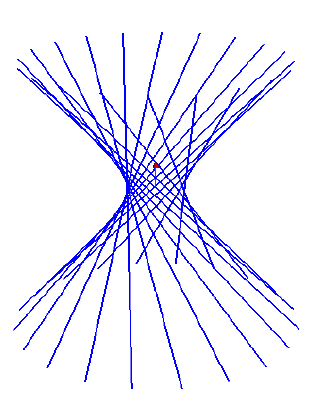
\includegraphics[width=0.5\textwidth]{regulus.png}
  \caption{A regulus}
  \label{fig:regulus}
\end{figure}

\section{Method and Approach}
The project can be roughly divided into three parts:
\begin{enumerate}
\item Becoming familiar with the field of projective geometry, Pl\"{u}cker
  coordinates, and the required algebra\"{i}c knowledge.
\item Implementing the GAViewer visualisation.
\item Researching the operations of 2D projective geometry in the geometric
  algebra of \rp.
\end{enumerate}
This division natually leads to three milestones:
\begin{enumerate}
\item got the mathematical background down
\item implemented visualisation
\item discovered something new and exciting
\end{enumerate}

The first part is rather straightforward, consisting mainly of reading papers,
books (\cite{dorst2009geometric}), and using GAViewer to build up intuition.
The second part is similarly well-defined; I will take a look at the code of
GAViewer and implement the missing regulus visualisation. The third (and main)
part is trickier. It will likely be a matter of mathematical manipulations and
experimentations until something useful rolls out. This process will be aided by
both the previous parts (as visualisation is incredibly useful when dealing with
geometry).

\section{Evaluation}
A quantitative evaluation is going to be hard or impossible. A qualitative
evaluation is more doable, if only of the form ``It didn't exist yet. Now it
does. That is good.'' Correctness of the result should be formally
provable due to the nature of the research. A comparison to the
existing complex homogeneous approach to 2D projective geometry used
by the Cinderella software is technically possible; however, it would be very
hard to find a suitable metric while eliminating interference from other
variables (e.g. a comparison on computational efficiency will likely depend more
on the used libraries than on the actual mathematical approach). A comparison of
this nature will not be in the scope of this research.
So in the end, the evaluation will consist of formal validation.

\section{Planning}
\begin{table}[h!]
  \centering
  \begin{tabular}{| l | p{9cm} |}
    \hline
    week & planning \\
    \hline
    \hline
    17     & finish obtaining mathematical intuition, write this proposal \\
    \hline
    18     & work on visualisation \\
    \hline
    19     & finish visualisation, start experimenting with the 2D geometry model \\
    \hline
    20, 21 & continue experimenting with the geometry \\
    \hline
    22     & prepare midterm presentation, do the Academic English assignment
    (impossible to estimate how long this will take), hopefully still have time for geometry  \\
    \hline
    23     & continue working with the 2D geometry \\
    \hline
    24     & Still doing geometry, nearing a finalisation of the work. Do the
    second Academic English assignment. \\
    \hline
    25     & Round-up the research, start documenting. \\
    \hline
    26     & Work for 14 hours a day, prepare report and
    finish presentation. \\
    \hline
  \end{tabular}
\end{table}
\FloatBarrier

\bibliographystyle{plain}
\bibliography{library}
\end{document}
